\documentclass[11pt,a4paper]{article}

\usepackage[margin=2.5cm]{geometry}
\usepackage{todonotes}
\usepackage{microtype}
\usepackage{amssymb,amsmath}
\usepackage{mathpazo}
\usepackage{accents}
\usepackage{longtable,booktabs}
\usepackage{pgf}
\usetikzlibrary{shapes.geometric}
\usetikzlibrary{matrix}
\usetikzlibrary{decorations.pathreplacing,angles,quotes}
\usepackage{natbib}
\usepackage{hyperref}
\usepackage[capitalise,noabbrev,nameinlink]{cleveref}
\hypersetup{
  pdftitle={Ouroboros Leios: design goals and concepts},
  pdfborder={0 0 0},
  breaklinks=true
}

\begin{document}

\title{Ouroboros Leios: design goals and concepts\\
       {\large \sc An IOG discussion paper}}
\date{Version 1.0, November 2022}
\author{Duncan Coutts        \\ {\small \texttt{duncan@well-typed.com}} \\
                                {\small \texttt{duncan.coutts@iohk.io}} 
  \and  Giorgos Panagiotakos \\ {\small \texttt{giorgos.panagiotakos@iohk.io}}
  \and  Matthias Fitzi       \\ {\small \texttt{matthias.fitzi@iohk.io}}
}

\maketitle

\section*{The purpose of Ouroboros Leios}

The motivation for Ouroboros Leios -- a new Ouroboros family variant -- is to
substantially increase throughput, while achieving at least as good security
properties as previous Ouroboros variants.

Existing variants of the Ouroboros blockchain algorithm are limited in the
throughput they can achieve -- both data throughput and CPU processing
throughput. They are not primarily limited by the resources available to each
node (network capacity or CPU performance), but by the nature of the data
dependencies and communication dependencies within the distributed algorithm.
Improving this requires a new algorithm design -- which is what Ouroboros Leios
is intended to be.

In addition, a new design provides an opportunity to incorporate other useful
modern features: tiered transaction fees with corresponding levels of service
priority, and faster chain synchronisation by removing the need to execute every
smart contract.

There are of course trade-offs in the design, in particular increased resource
use and increased transaction latency, and these are discussed.

The new Ouroboros Leios design is not a small or modular extension however. It
is a substantial extension of the Ouroboros Praos and Genesis designs, and the
changes to a practical implementation will also be substantial.

\section*{Intended audience}

The intended audience for this discussion paper is anyone in the Cardano
community with an interest in the performance of Cardano, or in the potential
future evolution of Cardano. The discussion is somewhat technical, so people
with a technical curiosity will get the most out of it.

\tableofcontents{}

\section{Existing throughput limitations}

A characteristic of network and CPU resources is that they are `use it or loose
it': time spent not using the available resources can never be regained. Thus
using these resources in a `spiky' fashion leaves the resources underutilised.

In the current deployed Ouroboros variant -- Ouroboros Praos -- we can observe
two main ways in which the algorithm does not fully utilise the network and
computational resources available on each node.

\subsection{Block diffusion is a fraction of overall block time}

In Praos, the time during which a block is forged and diffused across the
network is only a fraction of the overall average time between blocks. For
example with the parameters for the Cardano mainnet: blocks are produced
on average every 20 seconds, but the time to diffuse blocks across the network
is expected to remain within 5 seconds (this is the $\Delta$ parameter). This
means that on average three quarters of the time is spent idle. See
\cref{fig:praos-block-diffusion} for an illustration.

This can not be easily changed by tuning the parameters: the security argument
for Praos relies on the diffusion time ($\Delta$) being a fraction of the
average time between blocks. Intuitively, this is because if the diffusion time
became a large fraction of the average block time then there would be a higher
and higher proportion of `block battles', which would eat into the security
margins of the protocol. So for example, if the time between blocks was reduced,
then to maintain system security to the same level, the time allowable for
diffusion ($\Delta$) would also have to be reduced. This could only be reduced
by reducing the size of blocks, or by reducing the time budget per block for
executing scripts in transactions. The overall effect would be to reduce
throughput, even taking into account the more frequent blocks.

\begin{figure}[b]
\begin{center}
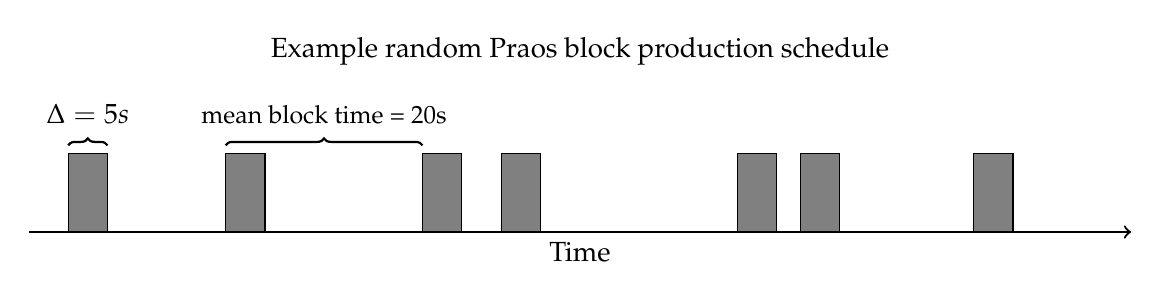
\begin{tikzpicture}

  \draw [fill=gray] (0.5,0) rectangle ++ (0.5,1);
  \draw [fill=gray] (2.5,0) rectangle ++ (0.5,1);
  \draw [fill=gray] (5,0) rectangle ++ (0.5,1);
  \draw [fill=gray] (6,0) rectangle ++ (0.5,1);
  \draw [fill=gray] (9,0) rectangle ++ (0.5,1);
  \draw [fill=gray] (9.8,0) rectangle ++ (0.5,1);
  \draw [fill=gray] (12,0) rectangle ++ (0.5,1);

  \draw[thick, ->] (0,0) -- node[below] {Time} (14,0);

  \draw (7, 2.3) node {Example random Praos block production schedule};

  \draw [thick, decorate, decoration={brace}]
        (0.5, 1.1) -- node[above=4pt] {$\Delta = 5s$} (1, 1.1);

  \draw [thick, decorate, decoration={brace}]
        (2.5, 1.1) -- node[above=4pt] {\small mean block time = 20s} (5, 1.1);

\end{tikzpicture}
\end{center}
\caption{Praos block diffusion time ($\Delta$) is a fraction of average time between blocks}
\label{fig:praos-block-diffusion}
\end{figure}

Notice that if the slot leader schedule were public rather than private, then
it would be possible to more densely pack diffusion periods: four times more
densely. This is the price we pay for the added security of a private slot
leader schedule in a traditional simple linear blockchain.

\subsection{Block diffusion underutilises resources}
\label{sec:diffusion-underutilises-resources}

The second, and more significant, way in which the available resources are not
utilised is within block diffusion itself: at any one moment while the new block
spreads throughout the network graph, only the nodes on the `information
wavefront' are active and utilising network and computational resources. To put
it another way: during block diffusion, before the block arrives at a node,
then that node is idle, and after it has downloaded, validated and forwarded
the block then it will return to being idle\footnote{There is additional work
after adopting a block to update and refill the mempool, which this the same
order of magnitude of work as the block validation itself.}.

See \cref{fig:serial-block-diffusion} for an illustration. Note how most time
for most nodes is spent idle. Something that is not immediately clear from the
illustration is that there is also relatively little overlap between CPU
activity and network activity on each node. This means the utilisation of each
resource is even less than it first appears.

\begin{figure}
\begin{center}
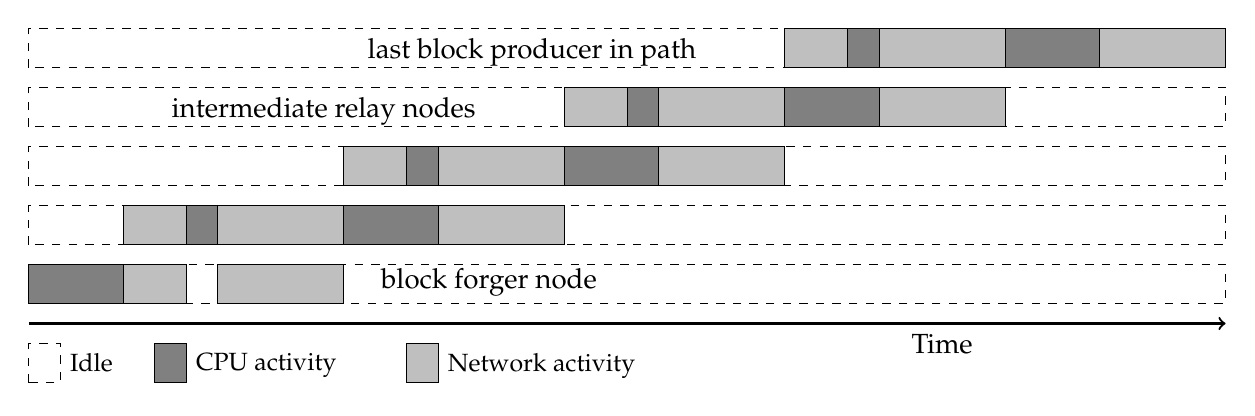
\begin{tikzpicture}

\begin{scope}[xscale=0.4, yscale=0.5]

\draw[dashed] (0,0.5) rectangle ++(38,1);
\draw[dashed] (0,2.0) rectangle ++(38,1);
\draw[dashed] (0,3.5) rectangle ++(38,1);
\draw[dashed] (0,5.0) rectangle ++(38,1);
\draw[dashed] (0,6.5) rectangle ++(38,1);


\begin{scope}[xshift=0cm, yshift=0.5cm]
  \draw[fill=gray]      (0,0) rectangle (3,1);
  \draw[fill=lightgray] (3,0) rectangle (5,1);
  \draw[fill=lightgray] (6,0) rectangle (10,1) node[right=10pt, yshift=2pt, anchor=north west] {block forger node};
\end{scope}

\begin{scope}[xshift=3cm, yshift=2cm]
  \draw[fill=lightgray] (0,0) rectangle (2,1);
  \draw[fill=gray]      (2,0) rectangle (3,1);
  \draw[fill=lightgray] (3,0) rectangle (7,1);
  \draw[fill=gray]      (7,0) rectangle (10,1);
  \draw[fill=lightgray] (10,0) rectangle (14,1);
\end{scope}

\begin{scope}[xshift=10cm, yshift=3.5cm]
  \draw[fill=lightgray] (0,0) rectangle (2,1);
  \draw[fill=gray]      (2,0) rectangle (3,1);
  \draw[fill=lightgray] (3,0) rectangle (7,1);
  \draw[fill=gray]      (7,0) rectangle (10,1);
  \draw[fill=lightgray] (10,0) rectangle (14,1);
\end{scope}

\begin{scope}[xshift=17cm, yshift=5cm]
  \draw[fill=lightgray] (0,0) node[left=1cm, yshift=-3pt, anchor=south east] {intermediate relay nodes} rectangle (2,1);
  \draw[fill=gray]      (2,0) rectangle (3,1);
  \draw[fill=lightgray] (3,0) rectangle (7,1);
  \draw[fill=gray]      (7,0) rectangle (10,1);
  \draw[fill=lightgray] (10,0) rectangle (14,1);
\end{scope}

\begin{scope}[xshift=24cm, yshift=6.5cm]
  \draw[fill=lightgray] (0,0) node[left=1cm, yshift=-3pt, anchor=south east] {last block producer in path} rectangle (2,1);
  \draw[fill=gray]      (2,0) rectangle (3,1);
  \draw[fill=lightgray] (3,0) rectangle (7,1);
  \draw[fill=gray]      (7,0) rectangle (10,1);
  \draw[fill=lightgray] (10,0) rectangle (14,1);
\end{scope}

\draw[dashed]         (0,-1.5) rectangle ++(1,1) node[anchor=north west] {\small Idle};
\draw[fill=gray]      (4,-1.5) rectangle ++(1,1) node[anchor=north west] {\small CPU activity};
\draw[fill=lightgray] (12,-1.5) rectangle ++(1,1) node[anchor=north west] {\small Network activity};

\draw[thick, ->] (0,0) -- node[below, xshift=4cm] {Time} (38,0);
\end{scope}

\end{tikzpicture}
\end{center}
\caption{Node (in)activity during pipelined block relay between five nodes}
\label{fig:serial-block-diffusion}
\end{figure}

\subsubsection{Quantifying the CPU resource utilisation}
Consider that validating a block is currently expected to take on the order of
50---100 milliseconds. So for each node -- at best -- this is only a few
hundred milliseconds out of 5 seconds for the overall $\Delta$ diffusion time.

This cost is roughly doubled by the validation of transactions entering the
mempool. This cost is not within the diffusion critical path, and can be spread
out over time. There are other costs and overheads, but this gives an indication of
the orders of magnitude involved.

\subsubsection{Quantifying the network resource utilisation}
The situation for network resource utilisation is more complex. There are two
important characteristics that affect the network resource use.
\begin{enumerate}
\item Nodes do not just send blocks to one downstream peer, they have many
      downstream peers. This increases the network resource use proportionally
      to the number of downstream peers.
\item Transmitting a block between two peers uses network resources only
      briefly: once on the sending peer to `serialise' the block onto the wire,
      and again briefly on the receiving peer to `deserialise' the block from
      the wire. Neither peer uses local network resources while the block is
      `in flight' between them.
\end{enumerate}
To quantify these effects, consider sending a 100kB block over a 1,000,000kB/s
network link\footnote{This is approximately 10GBit/s, but makes the example's
numbers clearer.} with 100ms of latency: the sending end will spend 0.1ms
serialising the block onto the wire, and then 100ms later the receiving end
will also spend 0.1ms deserialising the block off of the wire. If the same peer
has 1,000 downstream nodes then overall it will keep its local network interface
busy for 100ms out of the overall 5000ms $\Delta$ diffusion time.

Again, there are overheads but this gives an indication of the orders of
magnitude involved.

\section{Design goals}

\subsection{Throughput}

The primary design goal is to increase blockchain throughput by utilising a
significant fraction of each node's network bandwidth and CPU power, and do so
on an essentially continuous basis.

There are two primary measures and one derived measure of blockchain throughput
that we wish to increase:
\begin{enumerate}
\item data throughput, measured in bytes per second (typically as kilobytes per
      second, kB/s);
\item script throughput, measured in CPU seconds per wall-clock time in
      seconds\footnote{The unit is dimensionless, being seconds-per-second. We
      will nevertheless use a unit of `ms/s' because the seconds
      measure different things: CPU activity duration vs wall-clock duration.}
      (typically as CPU milliseconds per wall-clock second, ms/s);
\item transaction throughput, measured in transactions per second (TPS). This is
      not an independent measure but is derived from the other two.
      See \cref{sec:TPS} for a discussion of a TPS as a measure.
\end{enumerate}

To illustrate these two primary measures, let us consider what they are for the
existing Cardano mainnet. At the time of writing, Cardano mainnet blocks are
permitted to be a maximum of 88kB, and they are produced on average every 20
seconds. So the current data throughput is $88\text{kB} / 20\text{s} = 4.4\text{kB/s}$.

For comparison with the resources that could be available, consider that a
mid-to-high end server in a data centre would have a 10Gbit/s network interface.
If this server divides its bandwidth between 1000 peer nodes (and we allow for
around 20\% overheads) then this provides around 900kB/s of useful bandwidth
per peer. Or consider that a 10Mbit/s home broadband also provides around
900kB/s of useful bandwidth (given similar overheads).

For script throughput, at the time of writing Cardano mainnet blocks are
permitted to use up to a nominal\footnote{As calibrated on a reference machine.
Actual times will vary.} 40 milliseconds per block. So the current script
throughput is $40\text{ms} / 20\text{s} = 2\text{ms/s}$.

For comparison with a script throughput of 2ms/s, consider that a single CPU
core running flat out has 1000ms/s of processing time available. If multiple
cores are available and can be utilised then the CPU seconds available per wall
clock second will be greater than one.

It is worth noting that it is not sensible to try to utilise all of the network
and CPU resources at all times. Blockchain algorithms in the Ouroboros family
rely on being able to switch forks, which involves `catching up' on that fork,
and it is important to be able to catch up relatively quickly -- certainly
faster than real time. Furthermore, since Ouroboros uses random Poisson
distributions for the block production schedules, then there will naturally be
bursts and lulls of work. This places a limit on what fraction of resources can
be used in normal operation, so that catching up can be done sufficiently
quickly and so that the random bursts can be handled.

See also \cref{sec:how-fast} for a discussion of how fast, and how
resource-hungry we might want the Cardano mainnet to be.

\subsection{TPS}
\label{sec:TPS}

Transactions per second (TPS) is a measure of throughput that is often used to
compare different blockchain cryptocurrencies (and indeed other non-blockchain
data processing systems). TPS is a derivative measure, based on the data
throughput, the script execution time throughput and the size of the
transactions. For this reason we focus on the underlying measures of data and
script execution throughput. The resulting TPS can be calculated.

So while it is a goal for Ouroboros Leios to substantially increase throughput
measured in TPS, this will be a consequence of increasing the data and
script execution throughput, as discussed in the previous section.

It is also worth being aware that TPS is measure that is fraught with difficulty
in making fair comparisons between systems. This is because it depends crucially
on the size of a transaction and on how long any scripts within it take to run.
The simple way to make a system look good on TPS measures is to use as small a
transaction size as possible, with no (or very simple) scripts.

For example, suppose a blockchain has a data throughput of 500 kB/s. With 512
byte transactions this would yield 1000 TPS. For the same data throughput
but with transactions that all upload huge 16kB scripts, the result would be
just 31 TPS.

\subsection{Latency}

In the design of data processing systems it is often the case that there is a
trade-off between throughput and latency. Designs that process more transactions
per second often do so at the expense of an increase in the latency for
individual transactions.

In the case of blockchain systems, the usual definition of transaction latency
is the time between when a user submits a transaction into the system and when
it is included in a block that is available to most\footnote{More precisely
there will be latencies for reaching various proportions of users, such as 95\%
or 99\%.} other users. Note that this is not the time for the transaction to be
in a block that is stable with high probability.

For the Ouroboros Leios design we are prepared to make a reasonable sacrifice
in transaction latency in order to achieve a substantial improvement in
throughput.

\subsection{Security}

Some contemporary high throughput cryptocurrency systems make security
compromises to achieve high throughput, such as only being resistant to a 30\%
adversary. By comparison, existing versions of Ouroboros are resistant up to
a 50\% stake adversary, albeit with comparatively low throughput.

The goal for Ouroboros Leios is to achieve high throughput with no compromise
on security: to achieve the same or better formal security properties as
previous versions of Ouroboros.


\section{Design strategy}
\label{sec:design-strategy}

As discussed in \cref{sec:diffusion-underutilises-resources}, in Ouroboros
Praos, diffusing blocks over the network only uses a fraction of each node's
CPU and network resources. The fundamental reason for this is that a distributed
system of nodes is a \emph{parallel} system, but the Ouroboros Praos blockchain
algorithm is a (mostly) \emph{sequential} algorithm. Any sequential algorithm
executed on a parallel system will necessarily leave resources unused. The
algorithm for constructing the blockchain is necessarily sequential because the
structure of the blockchain itself is linear. It is linear in the sense that
the data dependencies in a valid chain are linear: each block depends on the
previous one. See \cref{fig:linear-blockchain} for an illustration.
Specifically, validating a block relies on computing the ledger state for the
block, which is computed as a function of the ledger state for the previous
block. Thus there is a direct data dependency between consecutive blocks, and
overall this forms a linear chain of data dependencies.

\begin{figure}
\begin{center}
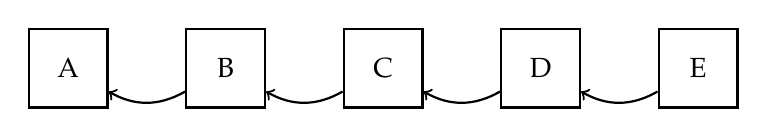
\begin{tikzpicture}

\begin{scope}[rectangle, thick, minimum height=1cm, minimum width=1cm]
  \node[draw] (block0) at (0,0) {A};
  \node[draw] (block1) at (2,0) {B};
  \node[draw] (block2) at (4,0) {C};
  \node[draw] (block3) at (6,0) {D};
  \node[draw] (block4) at (8,0) {E};

  \path[->] (block4) edge[bend left] (block3);
  \path[->] (block3) edge[bend left] (block2);
  \path[->] (block2) edge[bend left] (block1);
  \path[->] (block1) edge[bend left] (block0);
\end{scope}

\end{tikzpicture}
\end{center}
\caption{A traditional blockchain with its linear data dependencies. For
example: block B \emph{depends on} block A: the ledger state for B is computed
from the ledger state for A}
\label{fig:linear-blockchain}
\end{figure}

\subsection{A concurrent blockchain and a parallel algorithm}

Based on this observation, we can see that if we were to have a `concurrent
blockchain' with enough \emph{concurrent} data dependencies, then we may be
able to find a \emph{parallel}\footnote{We distinguish concurrency and
parallelism: concurrency is about data or events that are not sequenced with
respect to each other, whereas parallelism is about using more computer hardware
to compute more quickly.}
distributed algorithm for constructing the chain. If we can control the degree
of concurrency in the structure of the chain and the degree parallelism in the
algorithm, then this may allow us to increase the workload to the point where
we can use a substantial proportion of the resources available.

This is exactly what Ouroboros Leios attempts to do.

See \cref{fig:concurrent-blockchain} for an illustration of an imaginary pattern
of data dependencies between blocks. In the example in the illustration there
are up to three blocks at a time that are concurrent. One can imagine how this
pattern could be extended to higher numbers of concurrent blocks. The higher
the concurrency in the structure, the greater the opportunity to exploit more
hardware resources in parallel.

\begin{figure}
\begin{center}
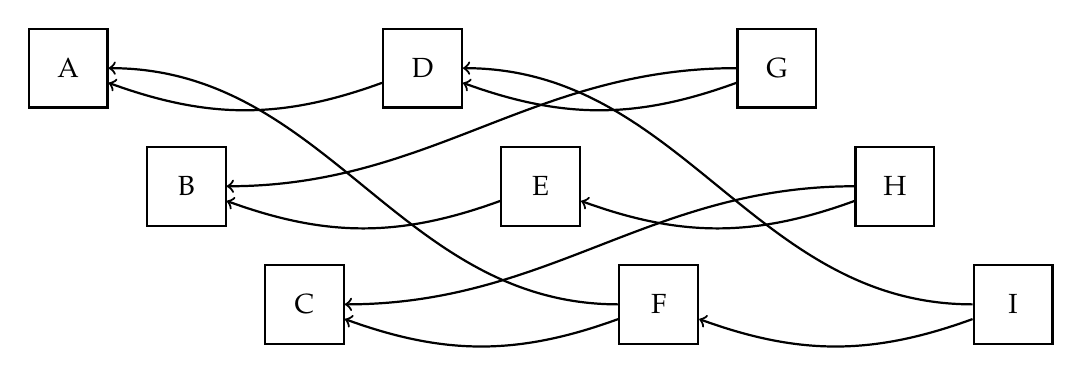
\begin{tikzpicture}

\begin{scope}[rectangle, thick, minimum height=1cm, minimum width=1cm]
  \node[draw] (block0) at ( 0.0, 3.0) {A};
  \node[draw] (block1) at ( 1.5, 1.5) {B};
  \node[draw] (block2) at ( 3.0, 0.0) {C};
  \node[draw] (block3) at ( 4.5, 3.0) {D};
  \node[draw] (block4) at ( 6.0, 1.5) {E};
  \node[draw] (block5) at ( 7.5, 0.0) {F};
  \node[draw] (block6) at ( 9.0, 3.0) {G};
  \node[draw] (block7) at (10.5, 1.5) {H};
  \node[draw] (block8) at (12.0, 0.0) {I};

  \path[->] (block8) edge[bend left=20] (block5);
  \path[->] (block7) edge[bend left=20] (block4);
  \path[->] (block6) edge[bend left=20] (block3);
  \path[->] (block5) edge[bend left=20] (block2);
  \path[->] (block4) edge[bend left=20] (block1);
  \path[->] (block3) edge[bend left=20] (block0);

  \path[->] (block8) edge[out=180, in=0] (block3);
  \path[->] (block7) edge[out=180, in=0] (block2);
  \path[->] (block6) edge[out=180, in=0] (block1);
  \path[->] (block5) edge[out=180, in=0] (block0);
\end{scope}

\end{tikzpicture}
\end{center}
\caption{An imaginary pattern of concurrent data dependencies between blocks.
For example block F depends on block A and C, but blocks D, E and F have no
dependencies between them.}
\label{fig:concurrent-blockchain}
\end{figure}

\subsection{Ledgers on a concurrent blockchain}
\label{sec:ledgers-on-a-concurrent-blockchain}

A somewhat concurrent blockchain structure has important implications for a
ledger built on that blockchain. The ledger would need to support the non-linear
blockchain structure, and this would not be possible for all ledgers. There are
a couple important issues:
\begin{enumerate}
\item It is important to understand the meaning of a ledger that is formed
      from joining the results of multiple concurrent blocks. This issue
      arises wherever multiple lines of data dependencies join. For example
      in \cref{fig:concurrent-blockchain}, block F depends on block A and C,
      which are concurrent with respect to each other. If mutually incompatible
      transactions are included in concurrent blocks, what is the interpretation
      of the resulting ledger?
\item Where a ledger is formed from concurrent blocks that are later joined,
      the computational costs need to be incurred predominantly with the
      concurrent blocks themselves and not with the point where they join.
      Otherwise most of the parallel advantage of a concurrent chain would be
      lost.
\end{enumerate}
These are not simple issues. Transactions in a ledger can depend on each other,
or be in conflict with each other. By definition, concurrent blocks cannot
depend on each other. So the challenge is what to do about transactions in
concurrent blocks that would depend or conflict with each other.

\subsubsection{Mostly independent transactions}
On the other hand the opportunity arises from the fact that \emph{most}
transactions -- that are `in flight' at the same time -- are independent of each
other, and independent transactions can be processed concurrently. Indeed the
ultimate limit on the degree of concurrency in the blockchain structure is the
extent to which in flight transactions are independent. The mixture of dependent
or independent in flight transactions is of course down to how the ledger is
used. One can imagine a specialised ledger managing a shared resource where most
transactions depend or conflict with each other, but for a general purpose
ledger (such as a `layer 1' platform) it is a reasonable expectation that most
in flight transactions are independent.

One non-solution is to delay the processing of transactions to the point where
the ledger from concurrent blocks are joined, and then process the transactions
in a linear order that can resolve their dependencies. This is a non-solution
because it squanders the CPU parallelism available, and will not be able to
fully utilise CPU time.

\subsubsection{Serialisability}
The `gold standard' in concurrent transaction processing (e.g.~in centralised
or distributed databases\footnote{For further reading see
\url{https://en.wikipedia.org/wiki/Serializability}}) is `serialisability'.
Concurrently processing a collection of transactions is serialisable if the
result of the concurrent processing is the same \emph{as if} the transactions
were processed serially in some order. Intuitively, this property means that we
have a clear interpretation of the ledger: we already understand what it means
to process a series of transactions in order, and so if the concurrent
processing gives the same result then that understanding is preserved.

\subsubsection{Optimistic concurrency control}
For general purpose ledgers where we can assume most in-flight transactions are
independent, we can take an `optimistic' approach to handle the few transactions
that do turn out to conflict:
\begin{enumerate}
\item We process multiple blocks of transactions concurrently.
\item Within each block the transactions are processed in order, so dependencies
      between transactions within a block can be handled normally.
\item When the results are joined, the blocks can put put into a linear order.
\item This gives rise to a linear order for the transactions: due to the blocks
      being put into an order, and transactions within blocks already being
      ordered.
\item Any conflicting transactions can now be discarded. Specifically, in a set
      of conflicting transactions, the first transaction is kept and the
      remainder are discarded.
\end{enumerate}
With this approach, conflicting transactions will reduce the effective
throughput, because they get processed only to be later discarded. However if
the rate of conflicts is not too high then this is a reasonable trade-off. Note
that it is crucial to avoid too many transactions artificially conflicting with
themselves by having the exact same transaction occur in concurrent blocks.

Importantly, to preserve parallelism, the detection and discarding of
conflicting transactions must be cheap relative to the cost of executing the
transactions (e.g.~running scripts and checking cryptographic signatures).

\subsubsection{UTxO style ledgers}
Fortunately UTxO-style ledgers are well placed to address these issues. This is
due to the fact that transactions in UTxO ledgers explicitly identify all of
their inputs and outputs up front, and those dependencies are complete. They are
complete in the sense that there are no other `side effects' of the transaction
other than the explicitly identified inputs and outputs. This makes it
straightforward to identify transactions that conflict with each other. It
also means that -- provided the dependencies between transactions are respected
-- the transactions can be reordered without changing the results. This makes
it possible to do the serialisation procedure outlined above correctly, and to
do so relatively cheaply. The correctness of this process can be formalised
mathematically.

It has long been touted that UTxO ledgers have potential advantages for
concurrency, but it has not typically been effectively exploited. It is
satisfying to find that this approach to concurrency can finally exploit those
advantages.

\section{Design outline}

All previous versions of Ouroboros use a simple traditional linear blockchain
structure. In contrast, Ouroboros Leios has an innovative new blockchain
structure with \emph{concurrent data dependencies}. As discussed in
\cref{sec:design-strategy}, this is the key to unlocking the opportunity for
increased parallelism and resource utilisation. Ouroboros Leios exploits the
concurrent data dependencies in the blockchain structure by using a
\emph{concurrent parallel distributed} algorithm for constructing the
blockchain.

Furthermore Ouroboros Leios is a \emph{scalable} algorithm, in the following
sense: the degree of concurrent data dependencies in the Leios blockchain
structure can be controlled, which directly influences the degree of
parallelism available in the execution of the distributed algorithm for
constructing it, and directly influences the resource utilisation and
throughput.

\subsection{Algorithm overview}
\label{sec:algorithm-overview}

There is new terminology to be aware of for the new kinds of objects involved
in the Leios blockchain structure and algorithm: \emph{input blocks},
\emph{endorsement blocks}, \emph{endorsement reports},
\emph{endorsement certificates}, and \emph{ranking blocks}. Each of these will
be covered as part of the algorithm overview, in summary in
\cref{table:block-types}, and again in detail in \cref{sec:blockchain-structure}.

\begin{table}
\begin{center}
\begin{tabular}{l p{3.5cm} p{3.5cm} p{3.5cm}}
\toprule
 & Ranking blocks & Endorsement blocks & Input blocks \\
\midrule
Acronym     & RB              & EB              & IB \\
Purpose     & consensus \newline ordering & IB existence \newline IB validity & carrying transactions \\
References  & one RB \newline many EBs & many IBs \newline zero or more EBs & one RB \\
Contains    & endorsement certificates &                 & transactions \\
Frequency   & 1 per 15---30s & 1 per 5---10 s & 1 per 0.2---2 s \\
\bottomrule
\end{tabular}
\end{center}
\caption{Summary of the different block types, their purpose and relationships}
\label{table:block-types}
\end{table}

\subsubsection{Creating input blocks}
Nodes can be elected (by private stake-weighted VRF lottery) to produce an
input block. When doing so, the node takes a sequence of transactions from the
mempool that are valid with respect to a recent point on the node's current
chain (which will be a ranking block, see \cref{creating-ranking-blocks}).
The node saves a reference to that same recent point on the chain. The
reference will be used later to ensure that other nodes will be able to
validate the transactions in the input block against the same ledger state.
The node packs the transactions into an input block, along with the reference
to the point on the chain, the VRF proof and signs the block.

\subsubsection{Relaying and validating input blocks}
The input block is made available to peer nodes and is relayed to all other
nodes. When other block producing nodes receive it, they validate the signature,
the VRF proof and the transactions within, using the ledger state corresponding
to the ranking block that the input block references (if available). Note that
input blocks do not depend on each other and they can all be relayed and
validated independently of each other. In principle, input blocks can be
generated at a high rate by tuning the VRF lottery threshold. This is the way
in which Ouroboros Leios can generate a lot of useful work to do, and -- just
as importantly -- can spread it out relatively evenly over time.

\subsubsection{Creating endorsement blocks}
Nodes can also be elected (by another separate private stake-weighted VRF
lottery) to produce an endorsement block. These gather up references to
recently seen valid input blocks that have not yet been included in other
endorsement blocks. They may sometimes also reference other recent endorsement
blocks that have not yet been included in a ranking block and where it would be
possible to create an endorsement certificate for them (which will be described
shortly in \cref{creating-endorsement-certificates}). They also include the
usual block signature and VRF proof. These endorsement blocks are the basis for
other nodes to issue endorsement reports on the endorsement blocks to say
whether all the input blocks referenced by the endorsement block actually exist
and are valid. Endorsement blocks are made less frequently than input blocks
but more frequently than ranking blocks. Note that it is ok if different
endorsement blocks are created concurrently by different nodes and reference
many of the same input blocks.

\subsubsection{Relaying endorsement blocks and creating endorsement reports}
The endorsement block is relayed to all other nodes in the usual way. When other
block producing nodes receive it, they stash it away until the time comes when
they may need to create an endorsement report for it. Endorsement blocks must
be checked and reported on a fixed number of slots after they are created. The
number of slots is a protocol parameter that is chosen to allow enough time for
the endorsement block to be relayed over the network, to reach all the nodes
that will perform the checks. Additionally, there is yet another private
stake-weighted VRF lottery where block producers can be elected as a reporter.
If a node has been elected as a reporter in the slot in which the endorsement
block must be checked, then it will check that all the input blocks referenced
by the endorsement block have already been seen and been verified\footnote{The
specification is that the check be performed \emph{as if} it were done at the
specific slot, but any equivalent check is acceptable. For example it is ok to
check the endorsement block earlier, but if not all input blocks have arrived
yet then the check has to be postponed.}. If the endorsement block references
other endorsement blocks then it must check that it has seen enough endorsement
reports for them that it would be possible to assemble an endorsement
certificate for them (see \cref{creating-endorsement-certificates} for details).
The node will then create a signed endorsement report and relay it to all other
nodes in the usual way. This report contains a signature, the usual VRF proof,
and a reference to the endorsement block in question. Note that very many block
producers are expected to be elected as reporters at once, so that there will
be lots of endorsement reports created and relayed around the network.

\subsubsection{Creating endorsement certificates}
\label{creating-endorsement-certificates}
The endorsement blocks and endorsement reports for those blocks are relayed
to the block producing nodes. Once enough endorsement reports for an
endorsement block have been collected then it becomes possible to create an
endorsement certificate for the endorsement block. The election of reporters is
calibrated so that there are enough of them, and they are fairly sampled from
the stake, so that we should be able to get `enough' endorsement reports. The
threshold for `enough' is based on a statistical argument that lets us conclude
(with a high degree of confidence) that \textgreater{}50\% of the stake
endorses the given endorsement block, and thus endorses the existence and
validity of all the input blocks referenced by the endorsement block (either
directly or via references to other endorsement blocks). When such a threshold
of endorsement reports can be collected then they can be assembled into an
endorsement certificate.

\subsubsection{Creating ranking blocks}
\label{creating-ranking-blocks}
Nodes can be elected (by yet another private stake-weighted VRF lottery) to
produce a ranking block. These gather up references to recent endorsement
blocks that have not yet been included in previous ranking blocks -- provided
that the node can construct and include an endorsement certificate for each one.
This will often mean that recently received endorsement blocks cannot yet be
included because not enough endorsement reports have yet arrived to produce a
corresponding endorsement certificate. Such endorsement blocks will typically
be included by the next ranking block. The ranking blocks also form the
`backbone' of the overall chain, with each ranking block referencing the
previous one. They also include the usual block signature and VRF proof.

Endorsement blocks can reference each other, but when they are included into a
ranking block, only the last in a chain needs to be included with an
endorsement certificate. This is because an endorsement certificate for an
endorsement block that references previous endorsements blocks implicitly
covers those previous endorsements blocks.

There is a limit on the number of endorsement blocks that can be directly
referenced in a ranking block (along with their corresponding endorsement
certificates). This is to limit the cost of validating a ranking block. If a
node has a choice about which endorsement blocks to include to fit within the
limit then it should choose the `biggest' ones, meaning the ones that (directly
or indirectly) reference the most input blocks.

\subsubsection{Relaying and validating ranking blocks}
A newly created ranking block is made available to its immediate peers via a
chain synchronisation protocol. Other peers receive and validate the extended
chain. The chain adoption rule here is \emph{almost} the same as in Praos: the
longest valid chain wins (with the usual rules about fair deterministic tie
breaking). Each ranking block is considered valid if it references a previous
valid ranking block and contains references to endorsement blocks with
corresponding valid endorsement certificates. This is sufficient to conclude
the chain is valid and adopt it. It is \emph{not} necessary to have also
already downloaded or validated all the endorsement blocks and the input blocks
they reference. The valid chain is adopted immediately, while constructing the
corresponding ledger state will lag behind.

\subsubsection{Constructing the ledger state for the ranking block chain}
After adopting a new chain, the node must construct the corresponding ledger
state. If necessary this may involve downloading any missing endorsement and
input blocks that were referenced by the new ranking blocks in the chain.

The ledger state must be constructed \emph{as if} all the transactions in all
the input blocks (indirectly) referenced by each ranking block were placed in
order and validated in that order (see
\cref{sec:serialisation-of-transactions-in-the-ledger} for details of the
order).

There is an important exception however: any transactions found to be in
conflict are treated as if they are \emph{not present in the ledger}. This
means that in a set of conflicting transactions, the first transaction (in the
transaction order) is accepted and the remaining ones are ignored. Note that
the ignored transactions are still physically in their original input blocks,
and thus take up space, but they are not logically part of the ledger.

Note that this specifies the outcome for the ledger layer, but not how it is
achieved. It is crucial for performance that the construction of the ranking
block ledger state involves less computation than fully validating all the
transactions in order. See \cref{sec:requirements-on-the-ledger-layer} for more
details.

\subsection{Blockchain structure}
\label{sec:blockchain-structure}

The Ouroboros Leios blockchain structure consists of three different kinds of
blocks, plus endorsement reports:
\begin{enumerate}
\item Ranking blocks (RBs)
\item Endorsement blocks (EBs)
\item Endorsement reports (ERs)
\item Input blocks (IBs)
\end{enumerate}
See \cref{fig:leios-concurrent-blockchain} for an illustration.

\begin{figure}
\begin{center}
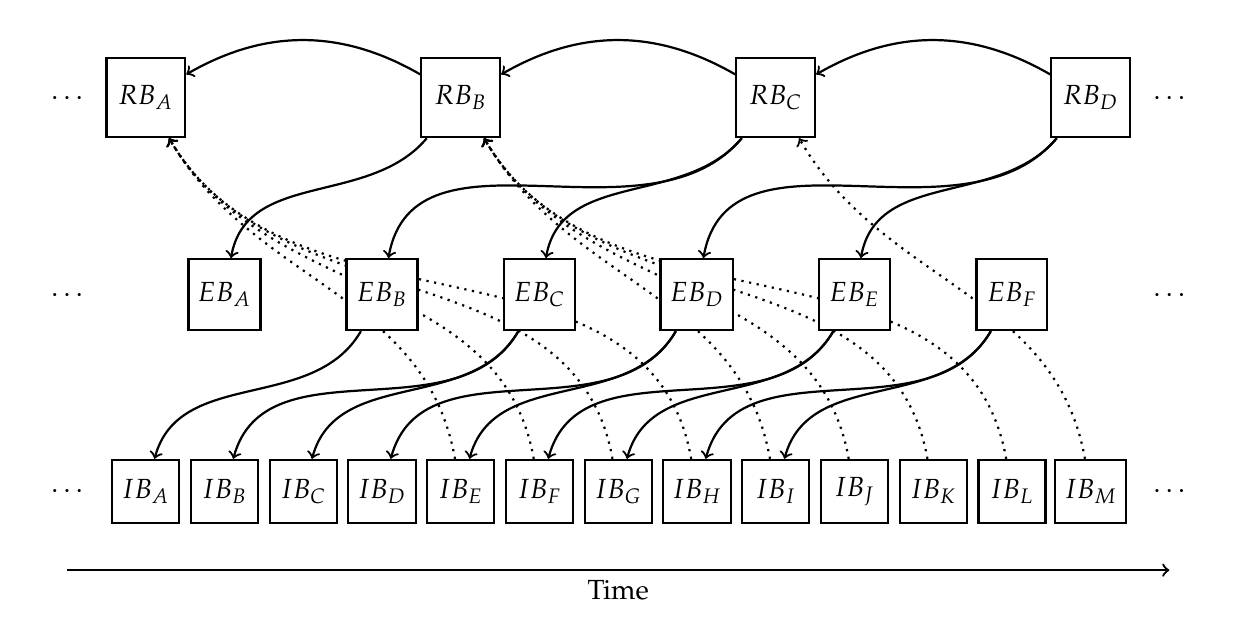
\begin{tikzpicture}

\begin{scope}[rectangle, thick, minimum height=1cm, minimum width=1cm, yshift=5cm]
  \node[]     (RB_0) at (-1,0) {$\ldots$};
  \node[draw] (RB_A) at ( 0,0) {$RB_A$};
  \node[draw] (RB_B) at ( 4,0) {$RB_B$};
  \node[draw] (RB_C) at ( 8,0) {$RB_C$};
  \node[draw] (RB_D) at (12,0) {$RB_D$};
  \node[ ]    (RB_E) at (13,0) {$\ldots$};
\end{scope}

\begin{scope}[rectangle, thick, minimum height=0.8cm, minimum width=0.85cm]
  \node[]     (IB_0) at (-1, 0) {$\ldots$};
  \node[draw] (IB_A) at ( 0, 0) {$IB_A$};
  \node[draw] (IB_B) at ( 1, 0) {$IB_B$};
  \node[draw] (IB_C) at ( 2, 0) {$IB_C$};
  \node[draw] (IB_D) at ( 3, 0) {$IB_D$};
  \node[draw] (IB_E) at ( 4, 0) {$IB_E$};
  \node[draw] (IB_F) at ( 5, 0) {$IB_F$};
  \node[draw] (IB_G) at ( 6, 0) {$IB_G$};
  \node[draw] (IB_H) at ( 7, 0) {$IB_H$};
  \node[draw] (IB_I) at ( 8, 0) {$IB_I$};
  \node[draw] (IB_J) at ( 9, 0) {$IB_J$};
  \node[draw] (IB_K) at (10, 0) {$IB_K$};
  \node[draw] (IB_L) at (11, 0) {$IB_L$};
  \node[draw] (IB_M) at (12, 0) {$IB_M$};
  \node[ ]    (IB_N) at (13, 0) {$\ldots$};
\end{scope}

\begin{scope}[thick, dotted, out=100, in=-60]
\path[->] (IB_E) edge (RB_A);
\path[->] (IB_F) edge (RB_A);
\path[->] (IB_G) edge (RB_A);
\path[->] (IB_H) edge (RB_A);

\path[->] (IB_I) edge (RB_B);
\path[->] (IB_J) edge (RB_B);
\path[->] (IB_K) edge (RB_B);
\path[->] (IB_L) edge (RB_B);

\path[->] (IB_M) edge (RB_C);
\end{scope}

\begin{scope}[rectangle, thick, minimum height=0.9cm, minimum width=0.9cm, yshift=2.5cm]
  \node[]                 (EB_0) at (-1,0) {$\ldots$};
  \node[draw, fill=white] (EB_A) at ( 1,0) {$EB_A$};
  \node[draw, fill=white] (EB_B) at ( 3,0) {$EB_B$};
  \node[draw, fill=white] (EB_C) at ( 5,0) {$EB_C$};
  \node[draw, fill=white] (EB_D) at ( 7,0) {$EB_D$};
  \node[draw, fill=white] (EB_E) at ( 9,0) {$EB_E$};
  \node[draw, fill=white] (EB_F) at (11,0) {$EB_F$};
  \node[]                 (EB_H) at (13,0) {$\ldots$};
\end{scope}

\begin{scope}[thick, bend right]
\path[->] (RB_D) edge (RB_C);
\path[->] (RB_C) edge (RB_B);
\path[->] (RB_B) edge (RB_A);
\end{scope}

\begin{scope}[thick, out=230, in=80]
\path[->] (RB_B) edge (EB_A);
\path[->] (RB_C) edge (EB_B);
\path[->] (RB_C) edge (EB_C);
\path[->] (RB_D) edge (EB_D);
\path[->] (RB_D) edge (EB_E);
\end{scope}

\begin{scope}[thick, out=240, in=75]
\path[->] (EB_B) edge (IB_A);
\path[->] (EB_C) edge (IB_B);
\path[->] (EB_C) edge (IB_C);
\path[->] (EB_D) edge (IB_D);
\path[->] (EB_D) edge (IB_E);
\path[->] (EB_E) edge (IB_F);
\path[->] (EB_E) edge (IB_G);
\path[->] (EB_F) edge (IB_H);
\path[->] (EB_F) edge (IB_I);
\end{scope}

\draw[thick, ->] (-1,-1) -- node[below] {Time} (13,-1);

\end{tikzpicture}
\end{center}
\caption{Data dependencies between blocks in Ouroboros Leios: each ranking block
(RB) references the previous ranking block and earlier endorsement blocks (EBs), which
reference still earlier input blocks (IBs). Input blocks also reference earlier
ranking blocks.}
\label{fig:leios-concurrent-blockchain}
\end{figure}

\subsubsection{Ranking blocks}
The purpose of ranking blocks is to achieve
consensus and an overall ordering. Each ranking block references the previous
ranking block, and references zero or more endorsement blocks (and includes
their corresponding endorsement certificates). Thus the ranking blocks form a
traditional linear blockchain, but instead of containing transactions, they
contain references to endorsement blocks. Indeed the ranking blocks form an
Ouroboros Praos chain, which enables the analysis and security results from
Ouroboros Praos and Genesis to be carried over.

As in Praos, ranking blocks are created using a private leader schedule, based
on VRFs and weighted by stake. This means that ranking blocks have a random
arrival pattern that follows a Poisson distribution, where the average time
between blocks can be tuned as needed. For global deployments the average time
between blocks would be expected to be similar to the 20s used on the existing
Cardano mainnet, but values in the range of 15---30 seconds could be
reasonable.

\subsubsection{Endorsement blocks}
The purpose of endorsement blocks is to help
agree on the existence and validity of input blocks. They gather up a bundle of
many input blocks to allow reporting on them as a bundle. This amortises the
cost of the construction and transmission of the reports over many input blocks.

Endorsement blocks are created using a private leader schedule, based on VRFs
and weighted by stake. The frequency of creation is expected to be tuned such
that there are approximately 2---4 endorsement blocks per ranking block.

\subsubsection{Endorsement reports and certificates}
The purpose of endorsement reports is -- in aggregate -- to demonstrate the
existence and validity of the bundle of input blocks referenced by the
endorsement block. In their aggregate form, with enough of them to
statistically represent \textgreater{}50\% of the stake, we call them an
endorsement certificate.

The endorsement certificates are what makes it possible to adopt a chain of
ranking blocks even if not all of the referenced endorsement and input blocks
have yet been seen: we know we will be able to find those blocks and we know
they will be valid. We know that on the basis that the endorsement certificate
demonstrates (to a high degree of confidence) that block producers representing
a majority of stake have seen the input blocks and checked that they are valid.
This also creates the opportunity for other blockchain consumers to skip
validation of input blocks and rely on the endorsement certificates to ensure
validity.

\subsubsection{Input blocks}
The purpose of input blocks is to carry the blockchain
payload: transactions. Each input block contains a sequence of transactions. It
also references a recent ranking block. This reference to a ranking block is to
make it explicit in which ledger state to use to validate the transactions in
an input block. Transactions within an input block can depend on each other.

Input blocks are also created using a private leader schedule using VRFs. They
are intended to be created at a high rate. The throughput of the Leios chain is
primarily determined by the input block creation rate and their maximum size.
Reasonable creation rates could be from one input block every few seconds, up
to several input blocks per second.

\subsection{Further algorithm details}

In addition to the overview in \cref{sec:algorithm-overview}, there are some
further details to the algorithm.

\subsubsection{Mempool sharding}
There is potentially a substantial amount of
concurrency available between multiple `in flight' input blocks, yielding
potentially a high data bandwidth. This could all be squandered however if most
concurrent blocks contained mostly the same transactions. This is a real danger.
It is to be expected that two nodes that create an input block at the same time
or a few seconds apart will have very similar mempool contents, and so a
na\"ive way of picking transactions from the mempool would be expected to
yield blocks with a high degree of overlap.

There are many potential solutions to this problem and further prototyping and
simulation will be required to pick the best design. The current best candidate
design is as follows. The transaction author assigns each transaction a `colour'
from a set. This is represented as a number from a limited range. Transaction
authors should assign this colour randomly, unless they want to submit multiple
dependent transactions in rapid succession, in which case they should assign
the subsequent transactions the same colour. Multiple cooperating transaction
authors creating dependent transactions may also be able to arrange this.

When a node comes to create an input block, it generates a random sequence of
colours, and then for each colour in turn it selects all the transactions from
the mempool with that colour. It keeps going, selecting transactions in this
way until the input block is full. This way, different nodes will typically
select different transactions, but dependent transactions can be kept together.

In the existing Cardano implementation, the mempool is sized to be proportional
to the amount of in-flight data: twice the block size. In Ouroboros Leios, with
all the concurrent input blocks, there is a lot more in in-flight data and
mempool sizes will need to be sized proportionally.

\subsubsection{Minimum and maximum times for inclusion}
There is a minimum time
between when an input block is created and when it is allowed to be referenced
in an endorsement block. Similarly there is a maximum time after which the
input block is no longer eligible to be referenced in an endorsement block.
Similarly there is a minimum and maximum times for endorsement blocks to be
referenced in ranking blocks.

These times are selected so that there is a reasonable time interval in which
the blocks are eligible for inclusion. The effect is that input blocks that are
not referenced by the first possible endorsement block can get referenced by
the next or subsequent endorsement blocks. This provides a reasonable degree of
protection from censorship, since many producers of endorsement blocks (fairly
sampled from the stake distribution) will have an opportunity to include each
input block before it expires when the maximum time bound is hit. This applies
similarly to endorsement blocks being included in ranking blocks.

The maximum bound is a defence against malicious block producer nodes that have
the right to produce many blocks but that delays doing so and then releases
them all at once. The maximum bound limits the size of such a flooding attack.
The other part of the defence is network prioritisation, discussed elsewhere.

The minimum bound serves two purposes: one is part of double signing protection
as will be discussed shortly, and the other is that it provides enough time for
the block to be relayed across the network. Providing enough time means there
is no unhelpful incentive for block producers to compete on being slightly
faster, and in particular no incentive for block producers to cluster close
together geographically, which would work against this important aspect of
decentralisation.

\subsubsection{Double signing protection}
The algorithm includes special measures 
to detect and handle the situation where a malicious or poorly-configured node
signs multiple different input or endorsement blocks in the same slot. Note
that this can happen accidentally when an SPO sets up an `active/active' or
`active/passive' failover system, if there is ever confusion resulting in more
than one node believing it is the active node, and thus signing blocks. This
protection is only needed for input blocks and endorsement blocks, not ranking
blocks, which is why this was not needed in Ouroboros Praos\footnote{The reason
ranking blocks, or indeed Praos blocks, do not need active double signing
protection is because they are part of chains, and the way chains are selected
naturally provides DoS protection. Nodes only download and adopt chains that
are better than their own current chain. Two chains of equal length ending in
two different blocks signed by the same peer are not better than each other in
the chain ordering, so nodes will select the first one they see and then not
select the second.}. Nodes keep track of recent input and endorsement blocks as
part of the normal procedures. If they receive a second block signed by the
same block producer for the same slot number, then this second block is added
to a tracking set and the block (or at least the header) is further relayed so
that most other nodes will also see the duplicate. Any subsequent duplicate
blocks from the same signer in the same slot are not relayed, to avoid denial
of service. This ensures that most block producing nodes will have seen that
there is a duplicate for a particular signer (though they may have different
blocks as evidence of this).

Now when a node comes to create an endorsement block, the rule is more
complicated than just selecting all available valid input blocks. Of course
input blocks that ended up in the double signature tracking set must not be
included. Furthermore, there must have been enough time to detect double
signing, and so the rule is that there a fixed number of slots after the input
block is created, before which it is not allowed to be included into an
endorsement block. The number of slots is a protocol parameter that is chosen
to allow enough time for any duplicate input block (headers) to be to be
relayed over the network. The rules for including endorsement blocks into
ranking blocks work analogously.

\subsubsection{Network resource prioritisation}
A block producer with significant stake could try to conduct a denial of
service attack by holding back a large number of blocks or endorsement reports
and then releasing them all at once. This is a particular concern for input
blocks and endorsement reports because these are created with relatively high
frequency. This would lead to a situation where there may be more blocks or
reports available to download than can all be downloaded at once in the short
term. It also provides an opportunity to choose what to download, or in what
order. Most legitimate blocks and reports will have recent slot numbers, while
those blocks and reports in the flood will have mostly older slot numbers.
Nodes therefore must always choose the recent blocks and reports if available,
and only choose older ones if they are the only ones available. The threshold
for `recent' here is a protocol parameter based on a reasonable upper bound on
the typical time it takes for blocks and reports to be relayed across the
network.

Additionally, when there are choices for what to download in limited bandwidth,
ranking blocks should be selected before other types of blocks and reports.

\subsubsection{Ledger state lags behind ranking blocks}
As noted briefly in the overview, it is possible to adopt a chain even though
not all of the referenced endorsement and input blocks have yet been downloaded
and verified. This has a few consequences that need to be explained. It means
a node's state has a current chain but it will in general only have a ledger
state for a recent ranking block and not necessarily the latest ranking block.
It also means the mempool will be revalidated against the last ranking block
for which we have a ledger state, rather than the latest ranking block.

A node in this `not fully caught up' state should prioritise downloading all
the missing endorsement and input blocks to try to catch up, because there are
certain activities it cannot participate in when not caught up. Nodes need the
ledger state for a ranking block to be able to validate input blocks that
reference that ranking block. Thus nodes that are not fully caught up cannot
create endorsement reports for new input blocks that reference a more recent
ranking block. Similarly, such a node that is elected to create an endorsement
block may have to pass up many input blocks if it cannot validate them. And
of course blockchain applications want to get the content of blocks, which
means getting access to the input blocks.

\subsubsection{Pessimistic mode}
Under extreme conditions when participation drops and the remaining active
block producers represent too small a fraction of stake, there may be too
few block producers creating endorsement reports to be able to make valid
endorsement certificates, and thus progress would stall. To degrade gracefully
in this situation and preserve liveness, the Ouroboros Leios switches to behave
much like Ouroboros Praos, which maintains liveness even with low stake
participation.

The way this works is that when a node is elected to create a ranking block, it
evaluates a predicate on the recent chain which then determines if the protocol
should be in `optimistic' or 'pessimistic' mode. The predicate is based on the
number of input blocks on the chain recently compared to the range that would
be expected. In optimistic mode, things proceed as described previously. In
pessimistic mode, the ranking block is created containing transactions directly,
without any endorsement blocks. This makes the block much like a Praos block.

\subsubsection{The time slot of a transaction}
Cardano transactions have a validity interval expressed in time slots. This
means that transactions may only be included onto the chain after some time
slot, and before another. This validity interval is the basis for the notion of
time in Plutus scripts.

In Ouroboros Praos the interpretation of the time slot is the slot of the block
in which the transaction is included. In Ouroboros Leios the situation is less
clear and there are multiple options with different trade-offs. Further
analysis is needed to decide on the best option.

One option is to declare that the interpretation of a transaction's time slot
is the slot of the \emph{input block} in which the transaction is included.
This would mean that a transaction can be included into an input block just
before the transaction's deadline, but it then takes some further time before
the input block is referenced in an endorsement block that is referenced in a
ranking block. This is in some sense reasonable: the transaction was submitted
and made it to a block producer on time, it is simply that the process of
building the chain takes some time afterwards to finish assembling everything.
An advantage of this is that it is simple to implement: the time interval check
can be performed along with all the other checks when transactions within an
input block are validated. A downside of this choice is that to be confident
that a transaction has \emph{not} arrived by a deadline would involve waiting
for the maximum time that input blocks are permitted to be included into
ranking blocks. Otherwise it is in principle possible that a transaction could
have been included in an input block, but that input block was delayed or
ignored by some block producers and ends up being included very late. How
reasonable this is depends on how long input blocks are allowed to hang around
before being included into a ranking block, which in turn is a protocol
parameter that needs further analysis to properly calibrate. Furthermore, this
option would mean that transactions appearing in the final chain do not
necessarily appear in time slot order: again because input blocks can be
delayed and included late.

Another option is to declare that the interpretation of the time slot is the
slot of the ranking block in which the transaction is included. This would have
the advantage that it is easy to know when a transaction has not arrived by a
deadline, as that would just involve waiting for the first ranking block after
a deadline. It would also mean that transactions would appear in time slot
order in the final ledger, since every transaction indirectly referenced by a
ranking block would be given the time slot of that ranking block. There are a
number of downsides too. There is the danger of transactions being included
into input blocks that later have to be ignored because they fall outside of
their validity interval, and unless carefully managed this could create a
denial of service opportunity. It complicates the ledger checks since it means
some checks have to be split and performed at different phases in the algorithm.
It also means that there is greater uncertainty with submitting transactions
before their deadline and getting them included reliably: delays in the
processing of endorsement or ranking blocks could mean that the transaction
misses its deadline, and this is outside the control of the transaction author.

\subsection{Algorithm commentary}

\subsubsection{Fast fork switching}
One of the motivations for the endorsement certificates scheme in Ouroboros
Leios is to address a tricky mismatch between theory and reality in the old
Ouroboros Praos design that would have become even worse in Ouroboros Leios.
The theory and security analysis for Ouroboros Praos relies on the assumption
that chains `diffuse' within $\Delta$ time slots (5s on Cardano). This is
something that the real implementation can do for single blocks and for short
forks of a few blocks. It is obvious however that the time to switch fork is
at least proportional to the length of the fork, and at some length that will
grow longer than $\Delta$ time slots. This issue is not a significant problem
in Cardano today with Praos, in part because blocks are not very large. It
would however become a big problem in Leios because it is designed to have
a lot more data and scripts on the chain and so the cost of validating all the
data referenced by each ranking block would be that much higher. This would
really violate the Praos assumption that chains can be diffused in $\Delta$
time, including switching forks. It could be violated for even fairly short
forks.

The endorsement certificates provide a way to switch forks on the ranking
block chain with comparatively little data needing to be download and
relatively little validation CPU work being needed. This restores the diffusion
$\Delta$ time assumption.

The ranking block payload is just the references to endorsement blocks, and
the endorsement certificates. These certificates are not tiny, but are not too
big. The ranking blocks can be adopted after verifying the endorsement
certificates but without having to yet download or verify all the endorsement
or input blocks.

\subsubsection{Lighter chain following}
\label{sec:lighter-chain-following}

The endorsement certificates also enable a novel feature for nodes that do not
produce blocks, such as relays and end user nodes. It allows them to catch up
and follow the chain \emph{without} having to execute smart contracts and
verify transaction signatures. They can reconstruct the ledger state for the
chain they are following by applying blocks, but in doing so they can skip
the verification of the execution of scripts and the verification of
transaction signatures. They can skip these checks because the endorsement
certificate says that nodes representing a majority of stake have already
verified the scripts execute as expected.

It is worth noting that in Cardano script execution does not affect the `result'
of a transaction -- since that is already provided in the transaction outputs --
it just affects whether the transaction is valid. If the transaction is known
to be valid then the resulting ledger state can be computed without executing
the scripts. The same is true for signatures on transactions.

The result of this is that it would be possible to follow the chain with less
CPU resources than otherwise. The chain data is still needed however. Though in
principle the transaction witnesses do not need to be downloaded.

\subsubsection{Lighter relays}
In Ouroboros Praos the resource cost of operating a relay is essentially
identical to the resource cost of operating a block producing node. The block
producing node does do some extra work, but it is relatively minor.

In Ouroboros Leios it is possible in principle to have relays that do less work
than block producing nodes. In particular, relays do not need to verify the
content of input blocks that they relay. For input blocks, endorsement blocks
and endorsement reports, their numbers are bounded provided the VRFs and
signatures are checked, and the double signing checks are performed. This is
sufficient to prevent DoS.

Relays must still follow the chain,  but they can use the technique described
above to do so relatively cheaply. Relays will still need the memory and disk
space to hold the ledger state, and the network bandwidth to serve all their
upstream and downstream peers, but should not need as much CPU processing power
as block producing nodes.

\subsubsection{Private VRF-based schedules}
The right to create the various objects (input blocks, endorsement blocks,
endorsement reports and ranking blocks) are all based on VRFs (verifiable
random functions). This is the same as the private leader schedule to create
ordinary blocks in Ouroboros Praos. The only difference is that there are now
four such schedules -- and crucially -- each one is independent of the other.
Each block producing node can produce any of the four different objects and
takes part in the corresponding schedule.

Each schedule works in the same way, based on a VRF, and weighted by the
delegated stake of the block producing node. The schedules for the four
different all have different thresholds, tuned to produce leaders at different
(average) rates. For example input blocks are made very frequently, while
ranking blocks would be made at much the same rate as Praos blocks are made now.

\subsubsection{Lower variance in block producer rewards}
Ouroboros Leios involves a lot more on-chain objects per epoch than in
Ouroboros Praos and thus many more opportunities for participation. The rewards
for participation will be similarly spread out over the different on-chain
objects.

In the existing Cardano deployment, there are on average 21,600 blocks per
epoch, and many block producing nodes are on the boundary of producing 0 or 1
block per epoch. This granularity creates high variance in the rewards each
epoch. Under Ouroboros Leios, we would expect a similar number of ranking
blocks per epoch as now, but there could be 10x--20x or more input blocks.

How rewards should best be spread out between the different objects is not yet
settled, but it is clear that there are far more objects contributing to
rewards. This would somewhat smooth out the epoch-to-epoch variance for block
producers with low stake, without necessarily affecting the expected
(i.e.~average) rewards.

\subsubsection{Slot and height `battles'}
In Ouroboros Praos, a so-called `height battle` occur whenever blocks are
created concurrently, meaning neither producer sees the other node's block
before making their own. This results in block producers loosing out since only
one of the blocks can end up in the final chain.

This situation looks quite different in Ouroboros Leios. There can still be
height battles for ranking blocks, but not for input and endorsement blocks,
nor for endorsement reports. Of course input blocks are \emph{intended} to be
created concurrently. They can all be gathered up and later included into the
ranking chain. The same applies to endorsement blocks.

The situation for ranking blocks is that while battles will still occur, they
should not be too frequent. In Praos, the only way to scale throughput --
bigger blocks -- also makes height battles more frequent. By contrast in Leios,
the size of ranking blocks is fixed even as throughput is scaled up, so the
typical time to relay a ranking block should remain fixed and relatively low.
This should keep the frequency of ranking block height battles fixed.

\subsubsection{Minimal incentives to be closer/faster}
Geographic decentralisation is an important component of network
decentralisation. The existing Cardano design tries to avoid incentives
towards geographic centralisation. This means trying to avoid rewarding block
producers for being faster, since the main way to be faster is to be physically
closer. This is due to the fact that network latency is a major component of
the time it takes for blocks to be relayed around the network. This is a
feature that is preserved in Ouroboros Leios.

For ranking blocks, ties are broken deterministically using a fair (uniformly
random) VRF. For input blocks and endorsement blocks, there is a minimum time
before these objects are allowed to be referenced and this time is set so that
there is adequate time to relay blocks across the network. Similarly,
endorsement reports are not used in a ranking block until some time later.

The effect should be that there is an incentive to not be very slow, but no
incentive to use especially high spec hardware or move physically closer to
other block producers. The `adequate' time to relay blocks across the network
will need to be set based on the minimum hardware requirements, as well as the
known network latencies. This is not expected to be a tight bound.

\subsection{Serialisation of transactions in the ledger}
\label{sec:serialisation-of-transactions-in-the-ledger}

There is a well defined overall order of transactions in the Leios blockchain.
As discussed in \cref{sec:ledgers-on-a-concurrent-blockchain}, this is
important to be able to provide a straightforward interpretation of the ledger.

The ranking blocks provide the overall order. Each ranking block (indirectly
via endorsement blocks) references a set of input blocks. The input blocks
referenced (indirectly) from a ranking block are ordered by their slot number.
Note therefore that it does not matter which endorsement block referenced which
input block (or if several did): all the input blocks referenced by all the
endorsement blocks in a ranking block are first considered as a set, and then
ordered by the slot number of the input blocks. There will often be ties due to
multiple input blocks being created in the same slot, and these ties are
resolved by a VRF\footnote{Note that this is a independent VRF from the input
block leader VRF, so the tie breaking is uniformly random.}. In the highly
unlikely\footnote{The VRFs used in Cardano have a 256bit output, so the chances
of a collision are tiny.} event of any ties remaining, the order is a free
choice by the author of the ranking block or endorsement block.

Note that this scheme does not guarantee that input blocks will appear in the
ledger in the order of their slot number, since it is possible for an input
block that is created earlier to end up in a later ranking block.

\subsection{Requirements on the ledger layer}
\label{sec:requirements-on-the-ledger-layer}

Ouroboros Leios imposes new constraints on the ledger layer. This is a direct
consequence of the new concurrency within the blockchain structure. Recall from
\cref{fig:leios-concurrent-blockchain} that the concurrent structure has both
`fan out' and `fan in' in the data dependencies between blocks. It has 'fan out'
in the sense that many input blocks depend on an earlier ranking block. This is
easy to handle using existing ledger functionality: each input block is
validated independently in a common initial ledger state. It has 'fan in' in
the sense that each ranking block depends (indirectly) on many input blocks.
This is where a new ledger operation is required: to assemble the ledger state
of a ranking block, based on the sequence of validated input blocks that
the ranking block (indirectly) references.

Intuitively what this operation needs to do is -- starting with the ledger state
of the previous ranking block -- to run through all of the transactions in the
ranking block in order and to perform some but not all of the normal ledger
checks. Specifically, it is not necessary to recheck things that do not depend
on the ledger state, which thus cannot be invalidated by a change in the ledger
state. As a simple example, the validity of transaction signatures do not
change if the ledger state changes. Any transactions that are found to be
invalid based on these checks are interpreted as if those transactions were
absent from the ledger. This will occur whenever transactions from independent input blocks
turn out to conflict with each other: for example if they spend the same inputs
or both withdraw funds from the same reward account. The resolution is that the
first transaction wins and subsequent ones are ignored. The later ones still
take up space in the input blocks, but they are not considered to be part of
the final ledger.

It is very important that this `reassembly' operation is not too expensive:
most of the validation work needs to be done when input blocks are validated
independently and not when they are reassembled into a ranking block. In
particular it is important that scripts do not need to be re-executed during
reassembly. Intuitively we expect it to be valid to skip script execution
because the ledger has been designed with great care to ensure that script
execution is deterministic. This means that when a transaction is checked in a
different ledger state, either the transaction is invalid (e.g.~due to missing
inputs) or if it is valid the script results will always be identical. If the
script result is always identical then the script execution does not need to be
repeated.

Of course intuition is not sufficient. The `determinism' property that would
guarantee the correctness of this reassembly operation needs to be formalised
and the ledger needs to be proved or otherwise carefully tested to ensure that
it satisfies this property.

Preliminary analysis suggests that the `pointer address' feature does not
satisfy this determinism property, and the feature will need to be removed in
order to support Leios. The pointer address feature was included in Shelley and
was intended to allow for shorter addresses, but the feature has proved hard to
use by wallets and has thus seen very little use. It is thus hoped that its
removal will not be too painful.

\subsection{Requirements on the network layer}

The Cardano network layer will need to be extended to support Ouroboros Leios,
but the fundamental architecture of the network layer will remain the same.
The specific set of `mini protocols' used to support the consensus algorithm
will need to be extended, but for example the way in which peers manager their
connections with each other in the peer-to-peer network will remain the same.

In particular, in Ouroboros Leios there are several new types of objects that
need to be relayed around the network: input blocks, endorsement blocks and
endorsement reports. Fortunately, the way these need to be transmitted all
follow an existing pattern: that of relaying of transactions, using
intermediate buffers (i.e.~the mempool). The most obvious design therefore is
to have three new mini-protocols for relaying the three new kinds of object,
each with corresponding buffers. One difference between relaying transactions
and the blocks and reports, is that the number of valid blocks and reports is
bounded (statistically) by their VRF-based leader schedules, whereas there is
no inherent bound on the demand for submitting transactions.

The chain synchronisation and block fetch protocols will still be used, but
just for ranking blocks. All the other blocks follow a relaying style.

For catching up on the chain it will also be necessary to be able to fetch
the other block types: input blocks and endorsement blocks. The block fetch
protocol will need to be suitably extended.

Due to the fact that Leios should be able to use a much higher fraction of
available network resources, it may be necessary to introduce more precise
control over prioritisation of different network transmissions: between
different block types, and between different peers.

\section{Development strategy}

Implementing Ouroboros Leios within Cardano will be a substantial undertaking
and will need to be approached carefully. To meet the performance goals, while
maintaining or improving the security and general quality will likely involve
a multi-year research and development effort.

Overall, the development strategy will be to do a lot of careful preparation,
prototyping, analysis and formalisation, before trying to integrate anything
into the existing codebase. This strategy will maximise the chances of success
and minimise the likelihood of problems occurring and causing delays in the
later implementation and integration stages.

Here are some of the major steps involved
\begin{itemize}
\item The Ouroboros Leios research design must be completed, including the
      security analysis, published and peer reviewed.
\item The various protocol parameters must be analysed based on the security
      results and calibrated. This may involve further design work if some
      parameters pose practical difficulties.
\item The Leios algorithm needs to be described in a suitable computer science
      formal language. This is different from the descriptions used in academic
      cryptography papers for security analysis. The purpose is to give a
      precise description of the functional behaviour, to help communicate the
      design to the engineering team, and later to help with testing the
      behaviour.
\item Performance is crucial for Ouroboros Leios and so much more performance
      prototyping and analysis will need to be done for Leios than for previous
      Ouroboros designs. This is to ensure that the performance characteristics
      are properly understood and to provide a degree of modularity in the
      performance of the design and implementation. Performance modularity
      means that it should be possible to give performance requirements for
      components of the system which -- if met -- will mean that the overall
      system meets its performance requirements. This is crucial to find and
      fix performance problems early, rather than only discovering once system
      level benchmarks are performed and then having difficulties in
      identifying which component or combination of components are the cause.
\item A detailed prototype implementation will be important to be confident
      that all the details of the design are included, understood and that they
      work together and achieve the goals. This prototype should be able to
      run in simulation and check some of the dynamic behaviour such as
      resource use, resource contention and some of the performance
      requirements.
\item Once a full prototype of the design has been made and validated, there
      will need to be detailed planning for how to adapt the existing Cardano
      implementation to support Ouroboros Leios, plus how to smoothly manage a
      hard fork from Ouroboros Praos to Leios.
\item In the ledger layer, there will be a lot of formalisation work to do to
      ensure that the ledger can correctly support the new operations.
\end{itemize}
All of this is needed before the implementation work starts, which itself
will of course take time. The implementation phase is also when the
property-based tests and component-level benchmarks are developed, based on
previously specified properties and performance requirements.

There will need to be an extended testnet phase to enable collaboration with
the authors of the many Cardano tools and applications, to support them with
the upgrade from Praos to Leios.

\section{Dependencies and relation to other features}

A full scale implementation of Ouroboros Leios in Cardano would depend on a few
other features.

\subsection{On disk storage of ledger state}
There is an ongoing project to transition the Cardano node's ledger state from
being fully in memory to being stored mostly on disk. This is necessary to
scale to larger ledger states, such as more UTxOs, more users, more scripts
stored in the UTxO etc. It will also reduce the RAM requirements for nodes
considerably once fully implemented.

The initial implementation of this feature uses a medium performance on-disk
backend, that is suitable for the existing level of throughput on Cardano. A
high performance backend is being planned. A suitably adapted variant of this
will be necessary for the high throughput requirements of Ouroboros Leios.

Note that a local SSD will become part of the minimum requirements for the
node\footnote{This is the case for all nodes, and thus also full-node wallets.},
but the RAM requirements should become relatively modest.

\subsection{Ouroboros Genesis}
Ouroboros Genesis is a modular feature that enables nodes to safely bootstrap
the blockchain from Genesis with minimal trust requirements. This feature is in
development to allow the IOG relays to finally be turned off, which along with
the peer-to-peer deployment, will complete the decentralisation of the physical
network.

Just as Ouroboros Praos+Genesis is a valid combination, Ouroboros Leios+Genesis
makes perfect sense too and provides the same benefits. Thus in some sense
Leios and Genesis are independent features. In practice Genesis will be
deployed by the time that Leios is available and so it would be a regression if
the Genesis feature were not included.

\subsection{Preparations in the ledger}
The existing Cardano ledger is well placed to fit the requirements of Ouroboros
Leios, but some preparation work will be required. In addition to the new
serialisation operations, the existing ledger rules must satisfy the
determinism property that we believe is necessary. The determinism property
also needs to be formalised and used to prove that the reassembly operation is
correct.

In particular the pointer address feature is believed not to satisfy this
property, and the feature will need to be removed. The remaining ledger rules
will need to be checked to verify that they do satisfy the determinism property.

\section{Future directions}

It is hard to anticipate directions for future research and development, but
there are a some issues that are already sufficiently clear that they are worth
a mention.

\subsection{Decreased latency}

The Ouroboros Leios design trades off increased latency for increased
throughput. In particular this means the latency of transactions being included
into the chain, and also the latency between transactions (in different input
blocks) that can depend on each other. One topic of research is to investigate
changes to the Leios design that would reduce the minimum latency between
dependent transactions. In particular, one promising idea is that instead of
input blocks referencing a previous ranking block as the context for validation,
they could instead use a `speculative' ledger state by referencing a ranking
block and an endorsement block. The referenced endorsement block should be one
that already has enough reports to construct an endorsement certificate, which
ensures that it is sufficiently available to all participants. The meaning of
the ledger state is then the ledger state of the ranking block, extended with
the ledger state formed from the serialisation of all the input blocks in the
endorsement block. Since endorsement blocks are created more frequently than
ranking blocks, this should reduce the overall latency between dependent
transactions.

\subsection{Horizontal scalability}

The Ouroboros Leios design provides what is classically called `vertical
scalability'. What this notion of scalability means is that as one increases
the computational and network resources of individual nodes, the throughput can
increase correspondingly. For example, classically one would describe database
servers or web servers as vertically scalable if their throughput increases
when run on ever `bigger' computers: more cores, faster cores and faster
I/O systems. In the Cardano context this would mean increasing the minimum
system requirements, e.g.~with more CPU cores or higher network bandwidth,
and then being able to use those resources to increase throughput, by
increasing the frequency of input blocks, or the size of input blocks.

The current Leios design does not however provide `horizontal scalability'.
This notion of scalability means that as one increases the number of computers
running the system, that the throughput can increase. For example a cluster of
web servers or database servers would be described as horizontally scalable if
the throughput of the cluster increases as more computers are added to the
cluster.

One direction of future research is to see if variations or extensions on the
Leios design could provide a degree of horizontal scalability. There are some
indications that this may be possible. For example, if instead of all block
producers validating all input blocks, they were just to validate the input
blocks that they need to report on, and if the mechanism for reporting would
shard input blocks around different reporters, then each reporter would only
need to look at a fraction of blocks. This would allow increasing the total
number of input blocks. This scheme would also have the positive benefit that
larger stake holders would be expected to validate more blocks than small
stake holders. This is fair in the sense that bigger stake holders would need
to dedicate more resources than smaller stake holders, but correspondingly
bigger stake holders can expect higher rewards.

There would be other aspects of the design that would also need to be revised
to be achieve a horizontally scalable design. In particular some mechanism
would need to be found for handling transactions on the submission side so that
not all nodes need to validate all transactions.

\section{The Cardano mainnet: how fast is too fast?}
\label{sec:how-fast}

If Ouroboros Leios can be implemented successfully and it is deployed on the
Cardano mainnet then the community will face a question it has not had to face
before: how to balance the trade-off between system performance and the
resource costs of participating. Higher system performance allows more use of
the system, but higher resource costs could put participation beyond the means
of many ordinary users. Put simply: the system could be too fast (and too
resource hungry) for most people to want to use it.

In a perfect world it would be possible to have high throughput and low
resource use for participants, but in the real world there is a trade-off:
increased throughput comes with increased resource use. Indeed the whole thrust
of the Leios design approach is to more fully utilise available resources as a
means to increase throughput.

For example, if the mainnet script execution budget were to be set to be a
substantial fraction of 4 cores of a typical x86 server, then correspondingly
the minimum hardware requirements for all validating nodes would need to be a
4-core x86 chip (or equivalent power). This would necessarily exclude people
running block producers or relays on their Raspberry Pis. More importantly it
would make full-node wallets effectively impractical for most users.

The Cardano community is not the only one to have faced this question. The same
topic arose in Bitcoin, albeit at lower levels of performance. The Bitcoin
community debated the merits of large vs small blocks. One of the arguments
made in favour of small blocks was ``to give end users the easy option to run a
node and therefore have a more decentralized system''\footnote{Quoting Till
Musshoff in \emph{The Bitcoin Block Size Wars Explained} \\
\url{https://www.bitrawr.com/bitcoin-block-size-debate-explained}}.

It is worth briefly reviewing what increasing the minimum resource requirements
might look like, and what the consequences would be and what mitigation might
be possible.

Suppose for the sake of argument that the system could be be run successfully
at a rate of 5 input blocks per second, with each input block being 100kB.

\paragraph{Disk space}
The example configuration gives a data rate of 500kB/s. At this rate, the disk
storage for the chain would grow at around 41 GB/day or 14.7 TB/year.

This is plainly out of the realm of practicality for home users to store the
entire chain. Multi-terabyte hard drives are not cheap, and even large desktop
computers can only hold a few hard drives.

\paragraph{Network bandwidth}
Network bandwidth is commonly measured in megabits per second, not bytes per
second. An application level bandwidth of 500kB/s has various protocol
overheads, so at the low level network will correspond to roughly 5 Mbit/s.
This would be a substantial fraction of most home users broadband connections,
and for many users would put them over usage caps.

\paragraph{Memory}
For this analysis we will assume that the current design to store the ledger
state on disk will be completed. Main memory will be required for indexes and
bloom filters for the large on-disk tables such as the UTxO. Initial estimates
suggest that a UTxO of 100 million entries (roughly the size of bitcoin) would
only need several hundred megabytes of memory for indexes and bloom filters.
The current design for on-disk storage involves maintaining the differences in
the on-disk tables in memory for the last K blocks, roughly 12 hours. This is
acceptable for the current Cardano data rates. At 500kB/s however it would need
a lot more memory. A rough calculation is that 500 kB could cover around 1000
small transactions, each with two UTxO inputs and outputs, which given the
memory representation of differences could need as much as 8 GB for 12 hours
worth of differences. This suggests that further design changes might be
necessary to keep even more of the state on disk.

\paragraph{CPU resources}
The CPU resources needed will depend directly on the budget that is set for
script execution. In principle it should be possible to push this high enough
to be able to saturate several CPU cores. Then the question is simply: what
minimum system requirements are acceptable.

It is worth noting, as discussed in \cref{sec:lighter-chain-following}, that
the Leios design does allow non-block-producer nodes to follow the chain
without having to validate the contents of input blocks. So the CPU resource
requirements for relays and end user nodes can be lower than for block
producing nodes.

\subsection{Mitigation}
It is clear that in a very high throughput configuration that Ouroboros Leios
would have resource requirements that are too high for most end users, at least
based on the current architecture of full node wallets and storing the whole
chain.

If such a high throughput configuration is desired, it may be necessary for the
vast majority of users to switch to light wallets.

It would also almost certainly be necessary for most end user full nodes to not
store the whole chain history. The node itself does not need the full chain
history (except currently when migrating the format of on-disk ledger state
snapshots), but some client applications do. For example, recovering a BIP44
wallet from a seed either requires the whole chain history or an index of all
addresses that have ever been used on the chain. Additionally, some scheme
would need to be developed so that most relays also do not need to store the
whole chain, but just the recent chain. The whole chain needs to be kept
somewhere of course and such a scheme would need to be able to assist nodes to
find where in the network the older parts of the chain are available.

Syncing the chain could also take an impractically long time. It may be
necessary to build in a feature to take snapshots of the chain state in such a
way that nodes can establish trust in a snapshot and continue following the
chain from there. Such a feature is currently being prototyped, under the code
name `Mithril'. It may be necessary for this to be a built-in feature to allow
a high performance configuration.

Each of these mitigations is a non-trivial feature in their own right. This
needs to be taken into account when planning for Ouroboros Leios integration,
if a truly high performance configuration is desired.

\end{document}
